%\begin{appendices}

\appendix
%\chapter*{ANEXOS}% If \appendix doesn't insert a \chapter
%\addcontentsline{toc}{chapter}{ANEXOS}% Print Appendix in ToC
\setcounter{section}{0}% Reset numbering for sections
\renewcommand{\thesection}{\Alph{section}}% Adjust section printing (from here onward)
	
	\section{Árbol de Problemas}
	%\chapter*{Árbol de Problemas}
	%\addcontentsline{toc}{section}{Árbol de Problemas}
	%\renewcommand{\thechapter}{A}
	\label{anexo1}
	\begin{figure}[h]
		\begin{center}
			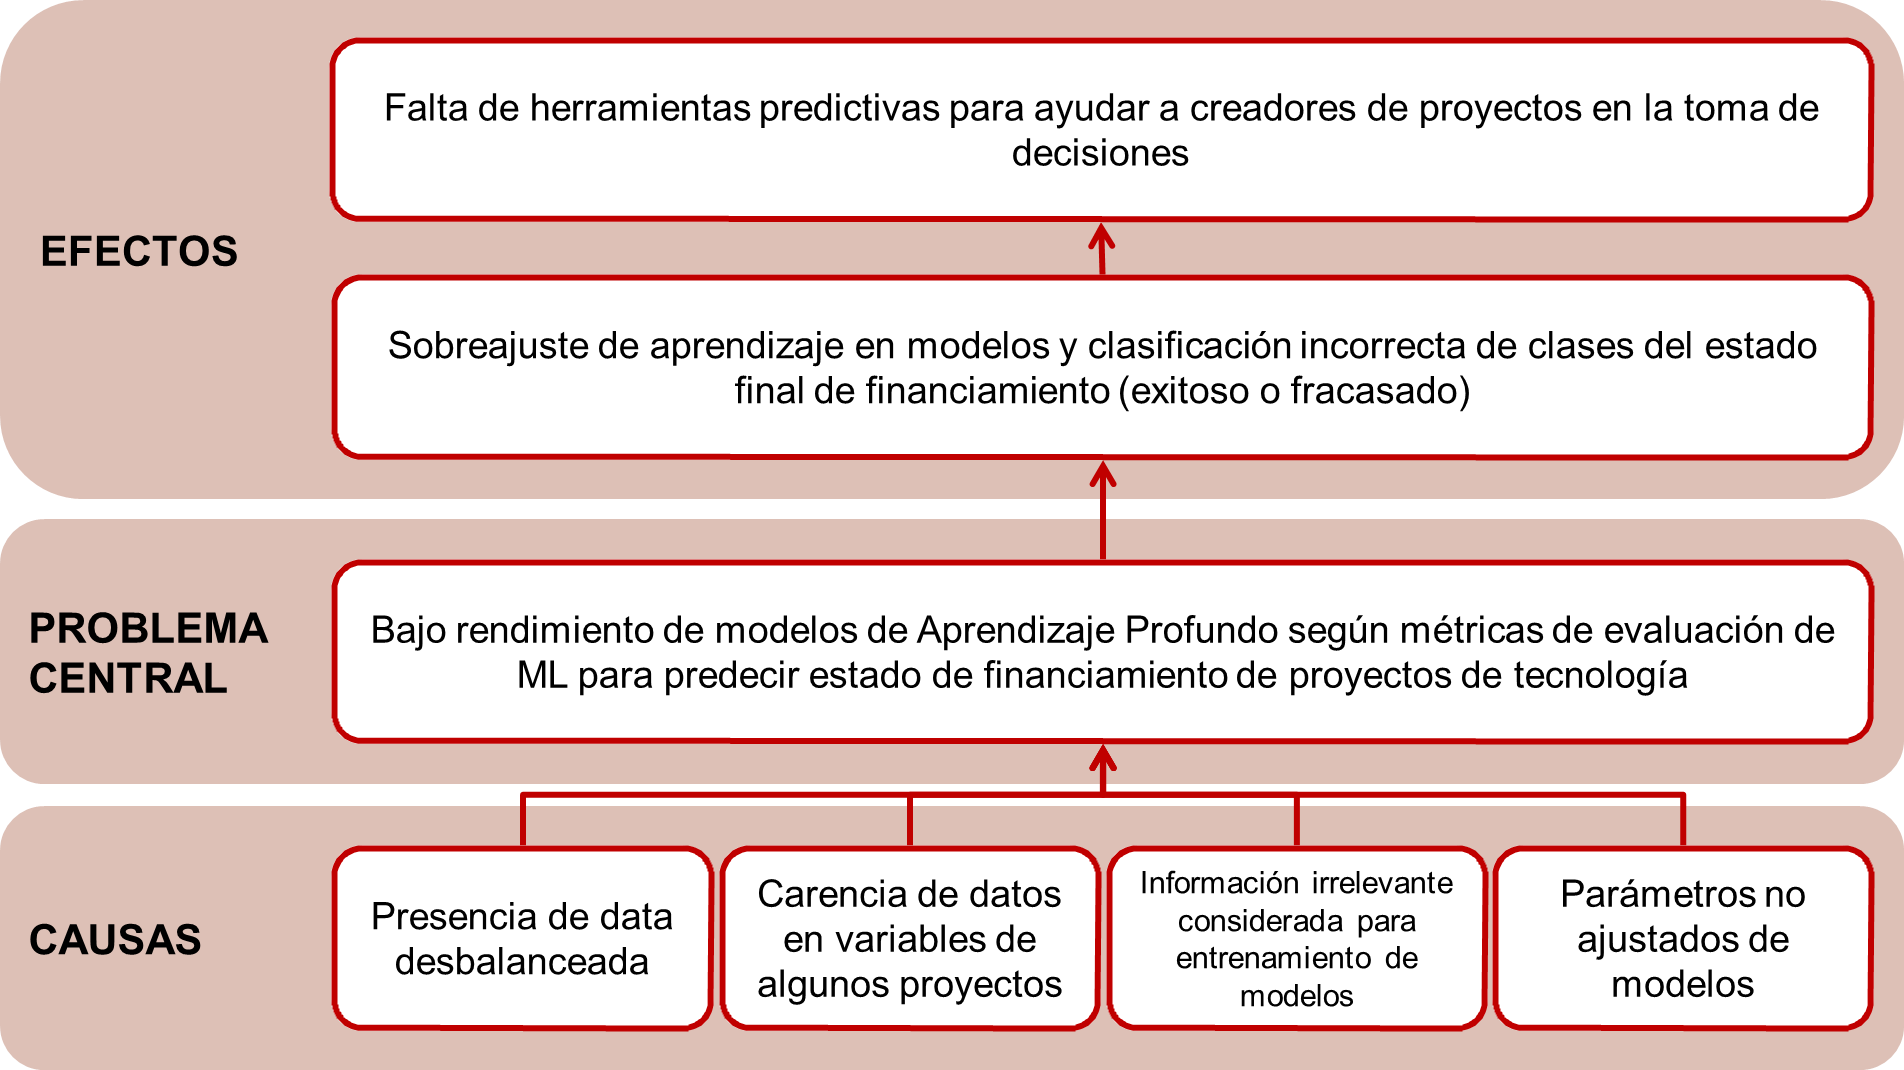
\includegraphics[width=1.05\textwidth]{anexos/arbol_problemas.png}
			%\caption{Fuente: Elaboración propia}
		\end{center}
	\end{figure}
	\clearpage
	
	\section{Árbol de Objetivos}
	%\chapter*{Árbol de Objetivos}
	%\addcontentsline{toc}{section}{Árbol de Objetivos}
	%\renewcommand{\thechapter}{A}
	\label{anexo2}
	\begin{figure}[h]
		\begin{center}
			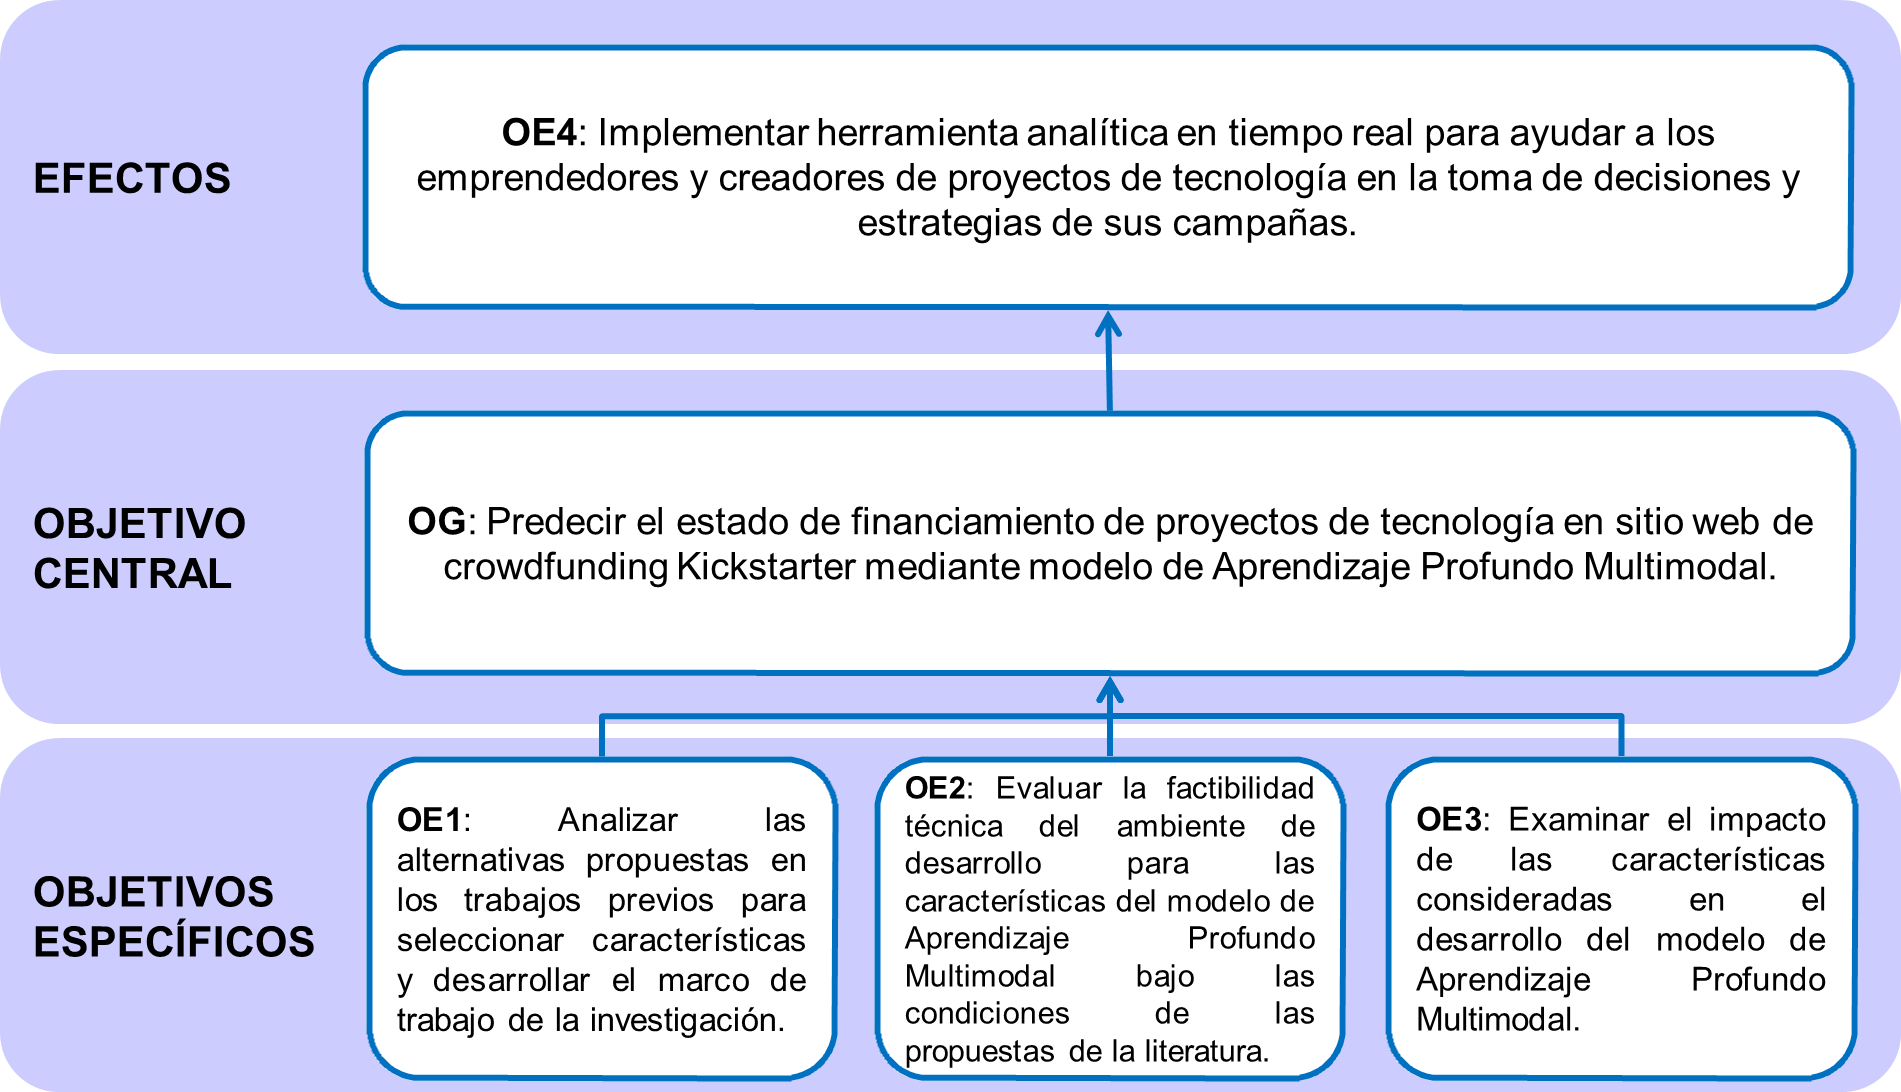
\includegraphics[width=1.05\textwidth]{anexos/arbol_objetivos.png}
			%\caption{Fuente: Elaboración propia}
		\end{center}
	\end{figure}
	\clearpage
	
	\section{Matriz de Consistencia}
	%\chapter*{Matriz de Consistencia}
	%\addcontentsline{toc}{section}{Matriz de Consistencia}
	%\renewcommand{\thechapter}{A}
	\label{anexo3}
	\begin{table}[h!]
		%\centering
		\small
		\begin{tabular}{ p{5.15cm}p{5.15cm}p{5.15cm} }
			\specialrule{.1em}{.05em}{.05em}
			\Centering{Problemas}& \Centering{Objetivos}& \Centering{Hipótesis}\\
			\specialrule{.1em}{.05em}{.05em}
			\Centering{Problema General}& \Centering{Objetivo General} & \Centering{Hipótesis General} \\
			\hline
			{\ProblemaGeneral} & { \ObjetivoGeneral} & {\HipotesisGeneral} \\
			\hline
			\Centering{Problemas Específicos}& \Centering{Objetivos Específicos} & \Centering{Hipótesis Específicas} \\
			\hline
			\vspace{0pt}{\Pbone} & \vspace{0pt}{\Objone} & \vspace{0pt}{\Hone} \\
			%\hline
			\vspace{0pt}{\Pbtwo} & \vspace{0pt}{\Objtwo} & \vspace{0pt}{\Htwo} \\
			%\hline
			\vspace{0pt}{\Pbthree} & \vspace{0pt}{\Objthree} & \vspace{0pt}{\Hthree} \\
			%\hline
			\vspace{0pt}{\Pbfour} & \vspace{0pt}{\Objfour} & \vspace{0pt}{\Hfour} \\
			%\hline
			\vspace{0pt}{\Pbfive} & \vspace{0pt}{\Objfive} & \vspace{0pt}{\Hfive} \\
			%\hline
			\vspace{0pt}{\Pbsix} & \vspace{0pt}{\Objsix} & \vspace{0pt}{\Hsix} \\
			\specialrule{.1em}{.05em}{.05em}
		\end{tabular}
		%\caption{Fuente: Elaboración propia}
	\end{table}
	\clearpage
	
	\section{Comparación de metodologías de antecedentes}
	%\chapter{Comparación de metodologías de antecedentes}
	%\addcontentsline{toc}{section}{Comparación de metodologías de antecedentes}
	\label{anexo4}
	%\begin{table}[htbp]
	\begingroup
		\renewcommand\arraystretch{0.5}
		\begin{longtable}{M{3cm}M{5.5cm}M{5.5cm}M{1.5cm}}
			\centering
			\small
			%% Se agrega tabularnewline para longtable
			\tabularnewline \specialrule{.1em}{.05em}{.05em}
			Autor & Título de la Investigación & Metodología & Grupo
			\\
			\specialrule{.1em}{.05em}{.05em}
			Chen, Jones, Kim \& Schlamp
			& KickPredict: Predicting Kickstarter Success
			& \setlist{nolistsep}
			\begin{itemize}[label={--},nosep,noitemsep,leftmargin=*,topsep=0pt,partopsep=0pt]
				\item Recolección de datos.
				\item Modelamiento.
				\item Evaluación.
				\item Despliegue.
			\end{itemize}
			& GG
			\\
			\hline
			Mitra \& Gilbert
			& The Language that Gets People to Give: Phrases that Predict Success on Kickstarter
			& \setlist{nolistsep}
			\begin{itemize}[label={--},nosep,noitemsep,leftmargin=*,topsep=0pt,partopsep=0pt]
				\item Recolección de datos.
				\item Pre-procesamiento de datos.
				\item Modelamiento.
				\item Evaluación.
				\item Despliegue.
			\end{itemize}
			& GE
			\\
			\hline
			Zhou, Zhang, Wang, Du, Qiao \& Fan
			& Money Talks: A Predictive Model on Crowdfunding Success Using Project Description
			& \setlist{nolistsep}
			\begin{itemize}[label={--},nosep,noitemsep,leftmargin=*,topsep=0pt,partopsep=0pt]
				\item Formulación del problema.
				\item Recolección de datos.
				\item Pre-procesamiento de datos.
				\item Modemiento.
				\item Evaluación.
			\end{itemize}
			& GD
			\\
			\hline
			Chen, Chen, Chen, Yang, Lin \& Wei
			& Will Your Project Get the Green Light? Predicting the Success of Crowdfunding Campaigns
			& \setlist{nolistsep}
			\begin{itemize}[label={--},nosep,noitemsep,leftmargin=*,topsep=0pt,partopsep=0pt]
				\item Recolección de datos.
				\item Pre-procesamiento de datos.
				\item Modelamiento.
				\item Evaluación.
			\end{itemize}
			& GF
			\\
			\hline
			Beckwith
			& Predicting Success in Equity Crowdfunding
			& \setlist{nolistsep}
			\begin{itemize}[label={--},nosep,noitemsep,leftmargin=*,topsep=0pt,partopsep=0pt]
				\item Recolección de datos.
				\item Pre-procesamiento de datos.
				\item Modelamiento.
				\item Evaluación.
			\end{itemize}
			&  GF
			\\
			\hline
			Li, Rakesh \& Reddy
			& Project Success Prediction in Crowdfunding Environments
			& \setlist{nolistsep}
			\begin{itemize}[label={--},nosep,noitemsep,leftmargin=*,topsep=0pt,partopsep=0pt]
				\item Formulación del problema.
				\item Recolección de datos.
				\item Pre-procesamiento de datos.
				\item Modelamiento.
				\item Evaluación.
			\end{itemize}
			& GD
			\\
			\hline
			Yuan, Lau \& Xu
			& The Determinants of Crowdfunding Success: A Semantic Text Analytics Approach
			& \setlist{nolistsep}
			\begin{itemize}[label={--},nosep,noitemsep,leftmargin=*,topsep=0pt,partopsep=0pt]
				\item Recolección de datos.
				\item Pre-procesamiento de datos.
				\item Modelamiento.
				\item Evaluación.
				\item Despliegue.
			\end{itemize}
			& GE
			\\
			\hline
			Sawhney, Tran \& Tuason
			& Using Language to Predict Kickstarter Success
			& \setlist{nolistsep}
			\begin{itemize}[label={--},nosep,noitemsep,leftmargin=*,topsep=0pt,partopsep=0pt]
				\item Recolección de datos.
				\item Modelamiento.
				\item Evaluación.
			\end{itemize}
			& GH
			\\
			\hline
			Kaur \& Gera
			& Effect of Social Media Connectivity on Success of Crowdfunding Campaigns
			& \setlist{nolistsep}
			\begin{itemize}[label={--},nosep,noitemsep,leftmargin=*,topsep=0pt,partopsep=0pt]
				\item Recolección de datos.
				\item Pre-procesamiento de datos.
				\item Modelamiento.
				\item Evaluación.
			\end{itemize}
			& GF
			\\
			\hline
			Kamath \& Kamat
			& Supervised Learning Model For Kickstarter Campaigns With R Mining
			& \setlist{nolistsep}
			\begin{itemize}[label={--},nosep,noitemsep,leftmargin=*,topsep=0pt,partopsep=0pt]
				\item Formulación del problema.
				\item Recolección y pre-procesamiento de datos.
				\item Exploración y extracción de datos.
				\item Modelamiento.
				\item Evaluación.
			\end{itemize}
			& GD
			\\
			\hline
			Yu, Huang, Yang, Liu, Li \& Tsai
			& Prediction of Crowdfunding Project Success with Deep Learning
			& \setlist{nolistsep}
			\begin{itemize}[label={--},nosep,noitemsep,leftmargin=*,topsep=0pt,partopsep=0pt]
				\item Recolección de datos.
				\item Exploración de datos.
				\item Pre-procesamiento de datos.
				\item Modelamiento.
				\item Evaluación.
			\end{itemize}
			& GE
			\\
			\hline
			Lee, Lee \& Kim
			& Content-based Success Prediction of Crowdfunding Campaigns: A Deep Learning Approach
			& \setlist{nolistsep}
			\begin{itemize}[label={--},nosep,noitemsep,leftmargin=*,topsep=0pt,partopsep=0pt]
				\item Recolección de datos.
				\item Modelamiento.
				\item Evaluación.
			\end{itemize}
			& GH
			\\
			\hline
			Jin, Zhao, Chen, Liu \& Ge
			& Estimating the Days to Success of Campaigns in Crowdfunding: A Deep Survival Perspective
			& \setlist{nolistsep}
			\begin{itemize}[label={--},nosep,noitemsep,leftmargin=*,topsep=0pt,partopsep=0pt]
				\item Formulación del problema.
				\item Recolección de datos.
				\item Pre-procesamiento de datos.
				\item Modelamiento.
				\item Evaluación.
				\item Despliegue.
			\end{itemize}
			& GA
			\\
			\hline
			Cheng, Tan, Hou \& Wei
			& Success Prediction on Crowdfunding with Multimodal Deep Learning
			& \setlist{nolistsep}
			\begin{itemize}[label={--},nosep,noitemsep,leftmargin=*,topsep=0pt,partopsep=0pt]
				\item Formulación del problema.
				\item Recolección de datos.
				\item Pre-procesamiento de datos.
				\item Modelamiento.
				\item Evaluación.
				\item Despliegue.
			\end{itemize}
			& GA
			\\
			\hline
			Chen \& Shen
			& Finding the Keywords Affecting the Success of Crowdfunding Projects
			& \setlist{nolistsep}
			\begin{itemize}[label={--},nosep,noitemsep,leftmargin=*,topsep=0pt,partopsep=0pt]
				\item Recolección de datos.
				\item Pre-procesamiento de datos.
				\item Selección de características.
				\item Modelamiento.
				\item Evaluación.
			\end{itemize}
			& GC
			\\
			\hline
			Chaichi \& Anderson
			& Deploying Natural Language Processing to Extract Key Product Features of Crowdfunding Campaigns: The Case of 3D Printing Technologies on Kickstarter
			& \setlist{nolistsep}
			\begin{itemize}[label={--},nosep,noitemsep,leftmargin=*,topsep=0pt,partopsep=0pt]
				\item Recolección de datos.
				\item Pre-procesamiento de datos.
				\item Selección de características.
				\item Modelamiento.
				\item Evaluación.
			\end{itemize}
			& GC
			\\
			\hline
			Shafqat \& Byun
			& Topic Predictions and Optimized Recommendation Mechanism Based on Integrated Topic Modeling and Deep Neural Networks in Crowdfunding Platforms
			& \setlist{nolistsep}
			\begin{itemize}[label={--},nosep,noitemsep,leftmargin=*,topsep=0pt,partopsep=0pt]
				\item Formulación del problema.
				\item Recolección de datos.
				\item Selección de características.
				\item Modelamiento.
				\item Evaluación.
				\item Despliegue.
			\end{itemize}
			& GB
			\\
			\hline
			Fernández-Blanco, Villanueva-Balsera, Rodriguez-Montequin \& Moran-Palacios
			& Key Factors for Project Crowdfunding Success: An Empirical Study
			& \setlist{nolistsep}
			\begin{itemize}[label={--},nosep,noitemsep,leftmargin=*,topsep=0pt,partopsep=0pt]
				\item Entendimiento del problema.
				\item Entendimiento de los datos.
				\item Preparación de los datos.
				\item Modelamiento.
				\item Evaluación.
				\item Despliegue.
			\end{itemize}
			& CRISP-DM
			\\
			\specialrule{.1em}{.05em}{.05em}
		\end{longtable}%
	\endgroup
	%\end{table}

%\end{appendices} 